\documentclass[a4paper,12pt]{jsarticle}
\bibliographystyle{junsrt}
\usepackage{ascmac}
\usepackage{empheq}
\usepackage{amsmath,amssymb}
\usepackage{bm}
\usepackage[dvipdfmx]{graphicx,color}
\usepackage[top=30truemm,bottom=30truemm,left=40truemm,right=40truemm]{geometry}
\usepackage{here}
\usepackage{comment}
\title{レーザー歪み計を用いた基線長安定化制御の提案}
\author{三代浩世希}
\begin{document}
\setcounter{tocdepth}{3}
\maketitle
\abstract{}
\tableofcontents

\section{防振装置の必要性}
重力波望遠鏡の鏡は地面振動雑音を低減するように振り子で吊られている。これにより共振周波数以上の帯域では鏡は慣性系に対して静止するようになる。そのため、より低周波で感度をもつために、より低い共振周波数の振り子を多段で組み合わせる工夫がなされている。しかしデザイン感度を満たす振り子であっても、干渉計が限られたダイナミックレンジの中で動作できるようRMSを小さくすることができなければ、望遠鏡として安定して動かすことはできない。

基線長変動のRMSは感度帯域より低周波の地面振動が大きく寄与している(図1)。0.2Hzのピークは脈動と呼ばれ、波浪が海底面を叩くことが原因である。脈動の振幅は波高と相関があり、その周期は浅瀬の深さに依存していることが知られている\cite{kedar2008origin}。更に低周波の$10^{-5}\, \mathrm{Hz}$のピークは地球潮汐と呼ばれ、地球と月の潮汐力によって引き起こされる。



\subsection{KAGRA}


\begin{figure}[H]
  \begin{center}
    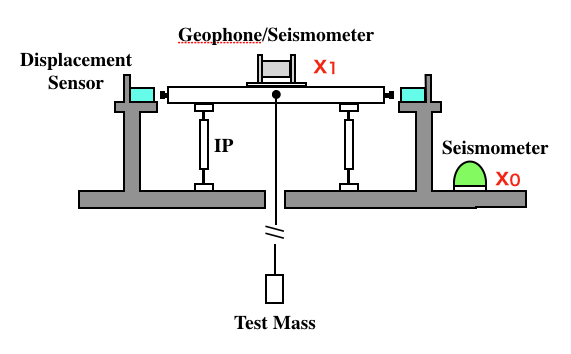
\includegraphics[width=11.5cm]{./img_pi.png}
  \end{center}
  \caption{}\label{img:img_pi}
\end{figure}

\subsection{FeedBackとFeedForward}

\begin{figure}[H]
  \begin{center}
    \includegraphics[width=11.5cm]{./img_ligo.png}
  \end{center}
  \caption{}\label{img:img_ligo}
\end{figure}

制御の目的は、PreIsolatorステージの変位$x_1$を目標値$r$に近づけつつ、外乱$x_0$からの影響を少なくすることである。現在LIGOで使われている制御\cite{matichard2015seismic}を図\ref{img:img_ligo}に示す。

\begin{eqnarray}
  x_1 &=& \frac{1}{1+G}P_{F}\left[\frac{P_{S}}{P_{F}}-C_{FF}\right]x_0 + \frac{G}{1+G}(L-C_{SC})x_0 \\
  &+& \frac{1}{1+G}P_{F}r \\
  &-& \frac{G}{1+G}Hn_{H} - \frac{G}{1+G}L(n_{SC}+n_{L}) - P_{F}C_{FF}n_{FF}  
\end{eqnarray}



\subsection{Hoge}
KAGRAのPreIsolatorは関口さんのD論から引用。\cite{sekiguchiD2016}
LIGOはここ。

\bibliography{./reference}

\end{document}
